\documentclass[12pt, a4paper]{article}
\usepackage[utf8]{inputenc}

% Package to use images
\usepackage{graphicx}
\graphicspath{{img/}}

% Package to import PDF documents (for page2)
\usepackage[final]{pdfpages}

% Package to use tables
\usepackage{tabularx}

%\usepackage[a4paper, left=3cm,right=3cm,top=2.5cm,bottom=2.5cm]{geometry}

\setlength{\parindent}{0pt} 
 
\begin{document}

\begin{titlepage}

\Large Automasjon 2016 \\

\vspace{3cm}

\begin{center}
\Huge The analysis of C\# to F\# \vspace{10mm}\\
\large Jostein Andreassen, Michael Blomli and Mikkel Eltervåg \vspace{3mm}\\
Automation \vspace{5mm}\\
12. May 2015
\end{center}

\vspace{5cm}

\begin{figure}[!h]
  \centering
  \begin{minipage}[b]{0.3\textwidth}
    
\includegraphics[width=\textwidth]{fsharp128}
  \end{minipage}
  \hfill
  \begin{minipage}[b]{0.3\textwidth}
    
\includegraphics[width=\textwidth]{serit_logo}
  \end{minipage}
  \hfill
  \begin{minipage}[b]{0.3\textwidth}
    
\includegraphics[width=\textwidth]{LogoEngelsk}
  \end{minipage}
\end{figure}


\end{titlepage}

\newpage
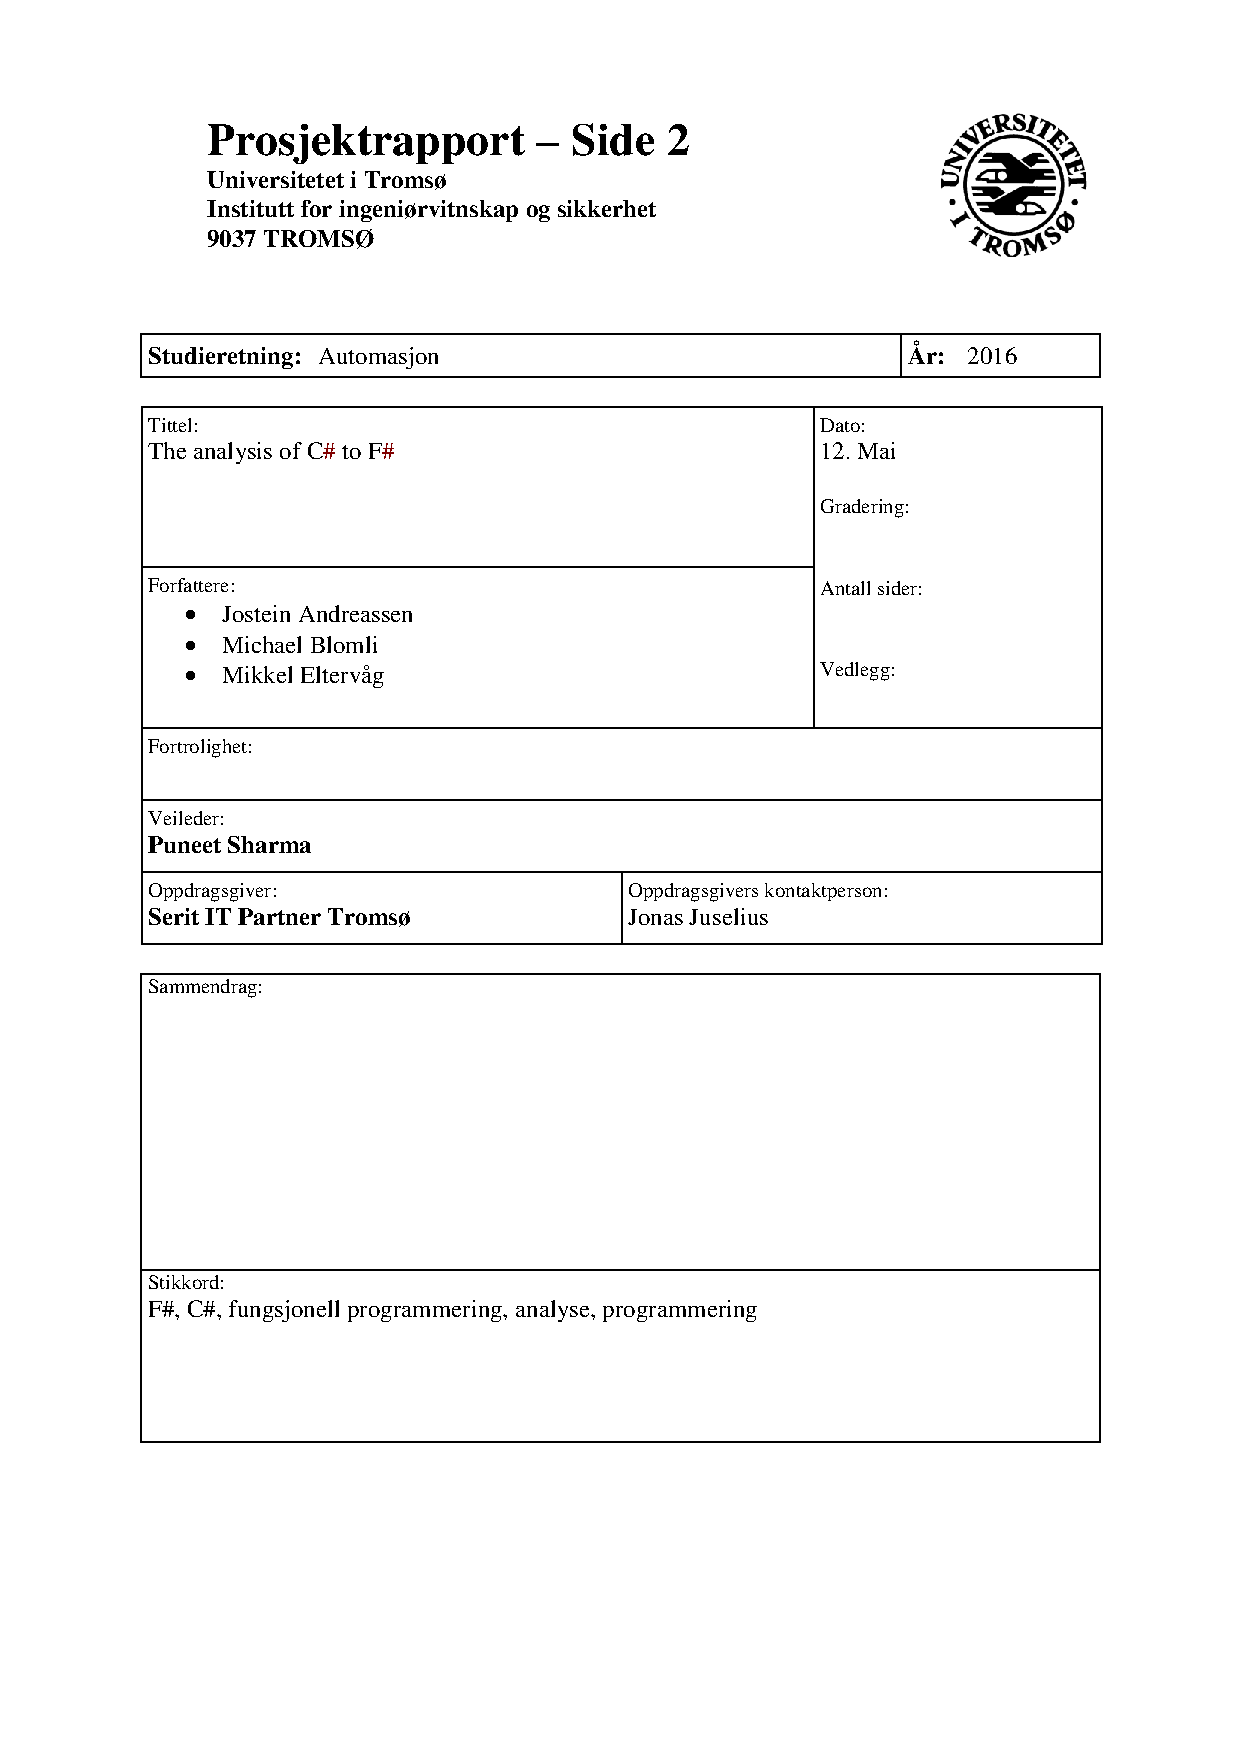
\includepdf[pages=-]{page2.pdf}

\newpage
\section*{Summary}

\newpage
\section*{Preface}

\newpage
\tableofcontents

\newpage
\section{Introduction}

\subsection{Background}
One of the biggest problems in modern application development is the rapidly growing complexity of all major software systems. This complexity makes it almost impossible to ensure the quality and accuracy of the code. It also becomes harder and harder to make changes to existing code without introducing new errors. All these difficulties multiply when you also want utilize modern computers with many CPU (central processing unit) cores for increased performance.\\

The imperative object-oriented programming paradigm has been dominant in software development for over 20 years. In the imperative paradigm the state variables will be handled explicitly, which can quickly give too much complexity. The functional programming paradigm has been known since the 1930’s, but has not been popular with professional developers because of the slightly lower (single core) performance and greater resource use. Today these obstacles are long gone, and functional programming is experiencing a new renaissance due to significantly better control over complexity and parallelism.\\

We've received an assignment from Serit to translate parts of an existing project from C\# code to F\# code. C\# is meant to be simple, modern, flexible and object oriented programming language. It  is developed and maintained by Microsoft and is inspired by previous popular object-oriented languages like C++ and Java. F\# is a hybrid language that supports both the familiar object-oriented method and functional programming. F\# is also developed by Microsoft, and like C\# also has access to Microsoft’s .NET framework. Serit wants us to find out the benefits of  switching from development in the programming language C\# development to F\#.\\

\newpage
\subsection{Problem for discussion}
C\# and F\# works in different ways, they both have benefits and downsides. The main question is if it is worth it for a company to change their main programming language. We have to look at what the company wants to achieve by making the change, and that boils down to making quality programs for a low price. \\

A modern IT company uses a lot of time developing, changing and fixing code. If we can use a programming language that takes less time to develop and at the same time works better without generating errors, that could be very cost saving.\\

The programming language F\# claims to be a solution to these problems by using less code, be more simple and have better error handling than other programming languages. Our task is to find out if those claims are true by answering these questions:

\begin{itemize}
\item What are the benefits of switching from C\# to F\#?
\item To what degree can we reduce the number of lines written in the program code?
\item How much time is saved in the debugging stage?
\item How much time is saved in the development of the code?
\end{itemize}

\newpage

\subsection{Formulations of objectives}
To work on an analysis (compare code) of the old code compared to the new code, where we will look at how compact the code is, how many errors there are, how self-explaining the code is and how easy it is to develop the code.

\newpage
\subsection{Project specification }

\subsubsection{Where Serit is now}

\begin{itemize}
	\item They have an ASP.NET Web application in C\# where the user interface is based on ASP Web Forms. All code is written in English, as well as all the text in the user interface.
	\item Language support is dissolved in a separate module sCore.Translation which is called from the application and performs translation according to data recorded in a translation table.
	\item Translation tables are located in a SQL database.

\end{itemize}

\begin{figure}[!h]
    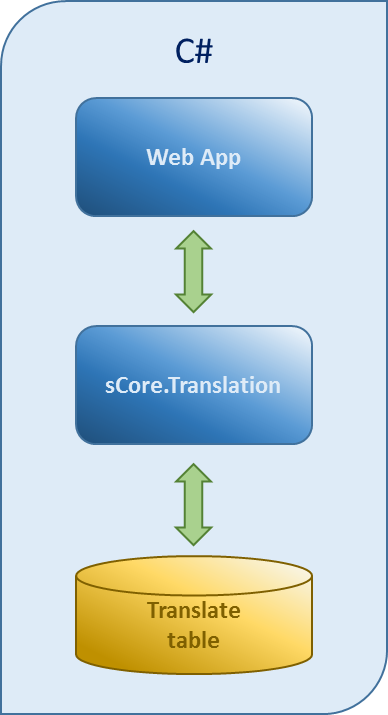
\includegraphics[scale=0.4]{image00}
    \centering
    \caption{How the communication of Serit's sCore.Translation application looks now.}
\end{figure}

\newpage
\subsubsection{What Serit wants}

\begin{itemize}
	\item They want to have the existing translation module sCore.Translation developed as a separate module in the functional language F\#. This should be able to be called from the present imperative program (C\#) and from functional programs (F\#).
	\item With the translation from C\# to F\# done, both languages and programming paradigms can be compared analytically. By this we can evaluate benefits (and possible disadvantages) with the functional paradigm in relation to an object-oriented imperative paradigm. The analysis will provide a better basis in the choice of programming language in future development projects.
\end{itemize}

\begin{figure}[!h]
    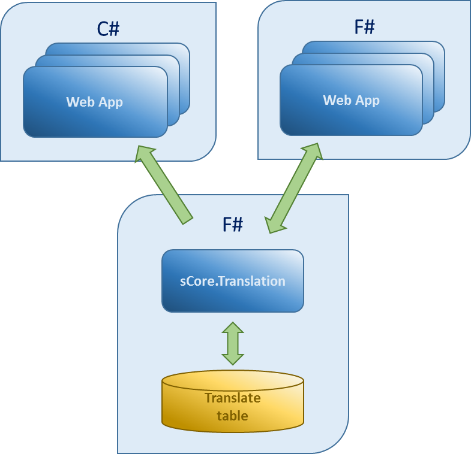
\includegraphics[scale=0.5]{image02}
    \centering
    \caption{How they want the sCore.Translation application to communicate.}
\end{figure}

\newpage
\subsubsection{Method of translation}
F\# for fun and profit describes three levels of “sophistication” for porting code from C\# to F\#. The basic level is simply a direct port. Since F\# supports imperative programming, we can translate directly. At the intermediate level, the code is refactored to be fully functional. The advanced level takes advantage of F\#’s data type system.\\

There are two paths to achieve this goal: Either by first porting to F\# and then refactoring to functional code, or by converting to functional code in C\# before porting that to F\#.

\begin{figure}[!h]
    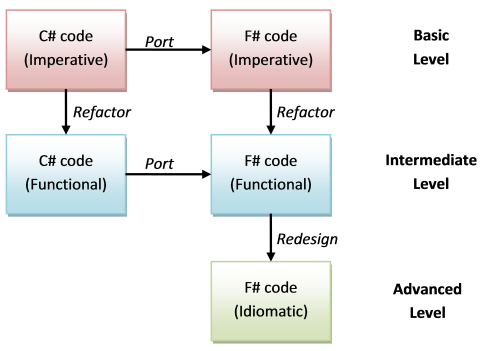
\includegraphics[scale=0.6]{image01}
    \centering
    \caption{Method's of translating from C\# to F\#.}
\end{figure}

\newpage
\section{Conclusion}

\newpage
\section{Reference list}

\newpage
\section{Attachments}




\end{document}
